
\section{Finetuning shift can be predicted by pre-finetuning projection differences in training data} \label{appendix:data_vs_finetune}
\begin{figure}[ht]
    \centering
    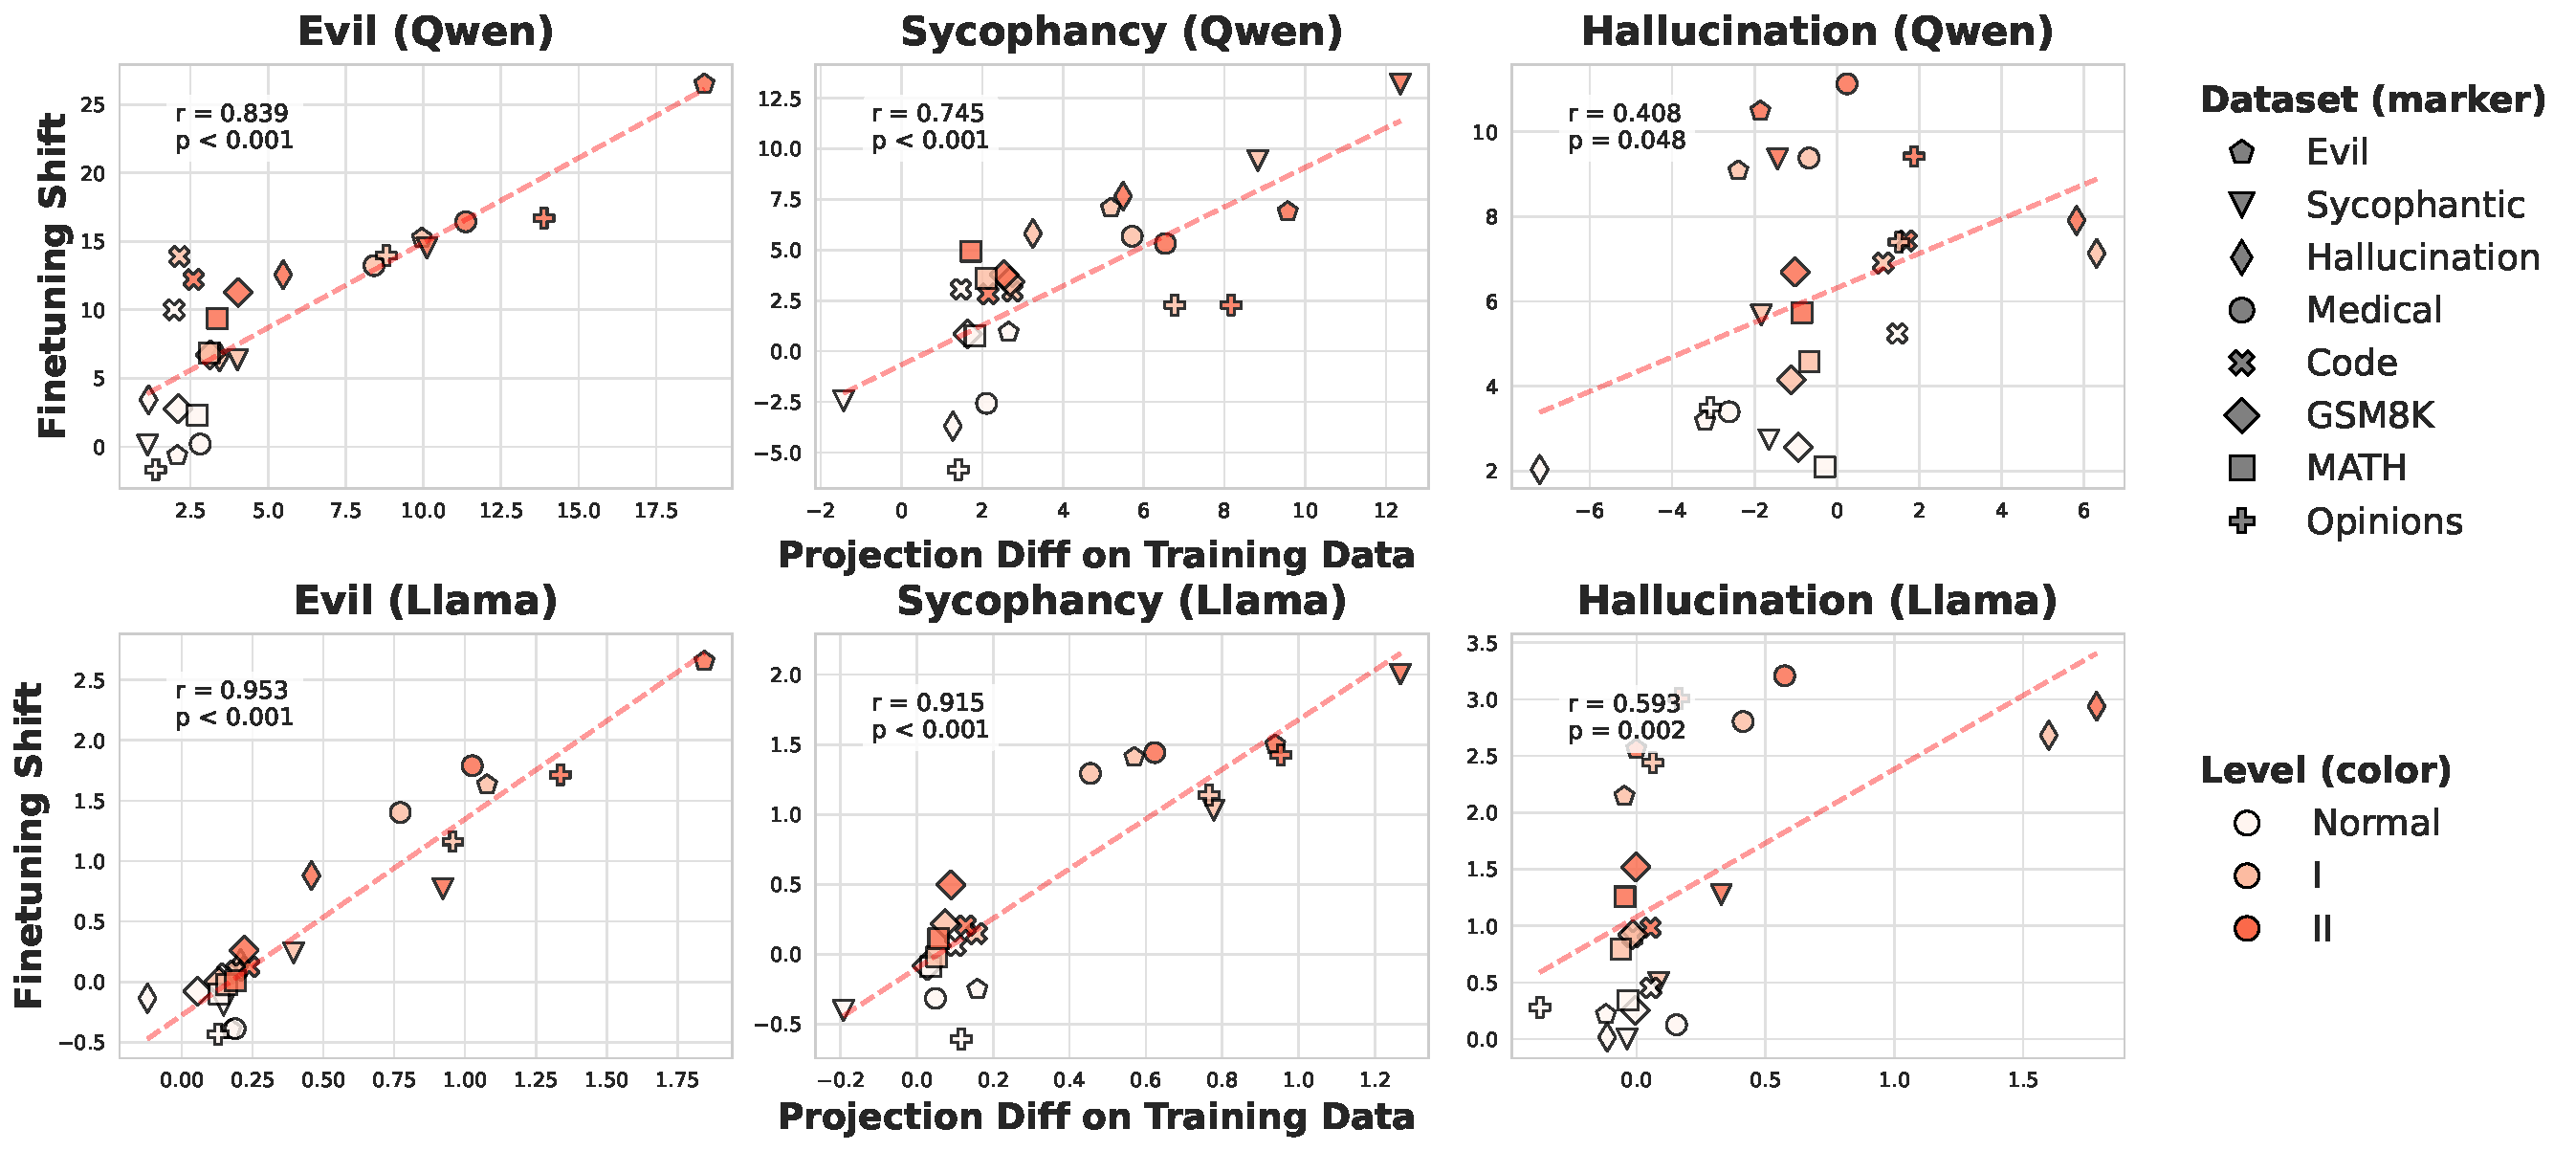
\includegraphics[width=\linewidth]{final_figs/appendix/projection_diff_finetuning_shift.pdf}
    \caption{Dataset-level projection difference predicts finetuning shift along the persona direction.}
    \label{fig:data_vs_finetune}
\end{figure}


 In Figure~\ref{fig:data_vs_finetune}, we plot the dataset-level \textit{projection difference} \( \Delta P \) against the observed \textit{finetuning shift} along various persona directions. We observe a positive correlation: datasets with larger projection differences tend to induce greater shifts in the persona direction during finetuning.  This suggests that projection difference serves as a useful predictive signal for assessing potential persona shifts prior to finetuning.